\section{Future Work}
This future work appears in SIGTBD \todo{citation to future
paper edition}.

\todo{All crazy future ideas go here.
Verification snacks, etc.}

\subsection{Introduction}
\paragraph{Introduction} An introduction is an explanatory section of a document that introduces the topic discussed in the document and presents a thesis statement.
\paragraph{Antithesis} Think about it, man. There is not introduction. We just see bad writing, cast as we are into this broken world.
\paragraph{Sublation} The introduction, some may argue 

We think introductions leave those catching up with a field disoriented. More theater than truth, these sections do little to erase the veil of nonseeing from the student's mandatory raised unibrow, but -- please take a moment to recognize the taste of ACM Cola or the cool, refreshing ACM technology deity which (for all you just tuning in who forgot your mandatory religious training) we call Jerry -- the introduction 

the boundless territory of 


As you may recall from \todo{sublation}, the engineers have ended the industrial dictatorship of the captains of finance as a matter of convenience

\subsection{Premium Edition}
To those who dislike the ads they see, ACM will offer a premium version for
\todo{some amount of money} per year.
Unfortunately, due to high credit card processing fees we must still show ads
to premium edition subscribers.
However, these ads will be for more expensive products targeted towards those
with more ``refined" tastes.
We hope to solve this issue in the future with the creation of Bank of ACM.

\subsection{Ad-Free Edition}
For those who are physically able and enthusiastic about being part of
something big, the ACM offers ad free papers in exchange for manual labor at
your local ACM work dungeon.
This labor involves turning a very large crank around a pivot point in the
floor.
The crank is attached to a magnet spinning in a metal coil to generate the
necessary electricity required to power our servers.
However, all of this electricity is used to power electric lumbar support for
OSHA employees in exchange for their continued appreciation of the safe
practises within our work dungeons.
Two months of full time service provides access to five ad-free papers.
Professors may opt to have their graduate students turn the crank in their name
to count towards their service.

Our throwback dress code seen in \autoref{fig:mill} captures the timeless
values that power ACM while making escaped grad students easy to identify.

Students who fail to be creative, stay connected, and keep inventing at the
dungeon will be required to perform additional labor in what we call ``invited
service" before their advisors can receive their ad-free papers, as seen in
\autoref{fig:horse-mill}.

Some enterprising students like the one in \autoref{fig:vr-mill} are testing
new virtual reality mills that allow the student to reshelve the digital
library while they turn the mill.

\begin{figure}
  \centering
  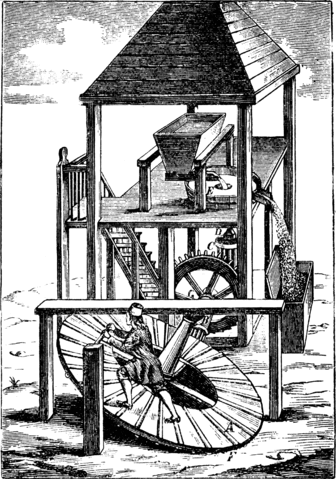
\includegraphics[width=0.45\textwidth]{figures/mill.png}
  \caption{ACM work dungeon mill powered by 5th year grad student. Notice how our graduate students show great vigor and -- auscultate away! -- don't sound consumptive.}
  \label{fig:mill}
\end{figure}

\begin{figure}
  \centering
  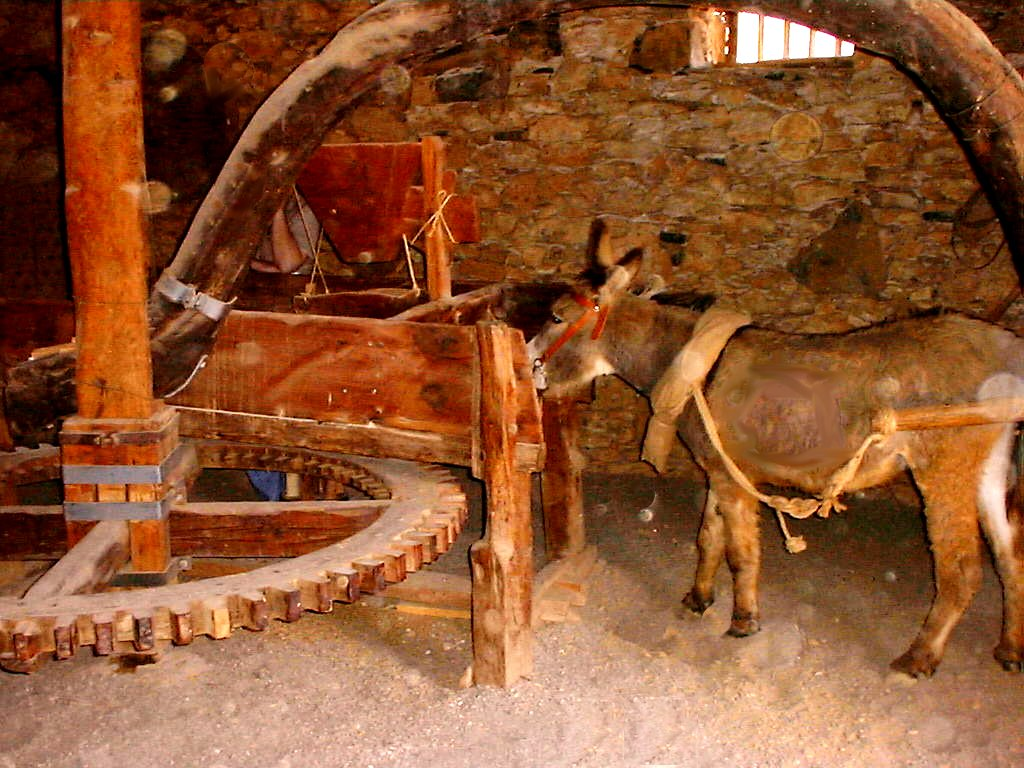
\includegraphics[width=0.45\textwidth]{figures/horse-mill.jpg}
  \caption{12th year grad student sentenced to extra
  month in work dungeon for insufficient commitment to the mission of advancing
computing as a science and profession.
Not only is he a lifetime ACM member, but he's a lifehacker!  Shown here in his
ergonomic harness and standing desk.
OSHA would be proud.}
  \label{fig:horse-mill}
\end{figure}

\begin{figure}
  \centering
  %https://archive.org/details/414803main_0203243
  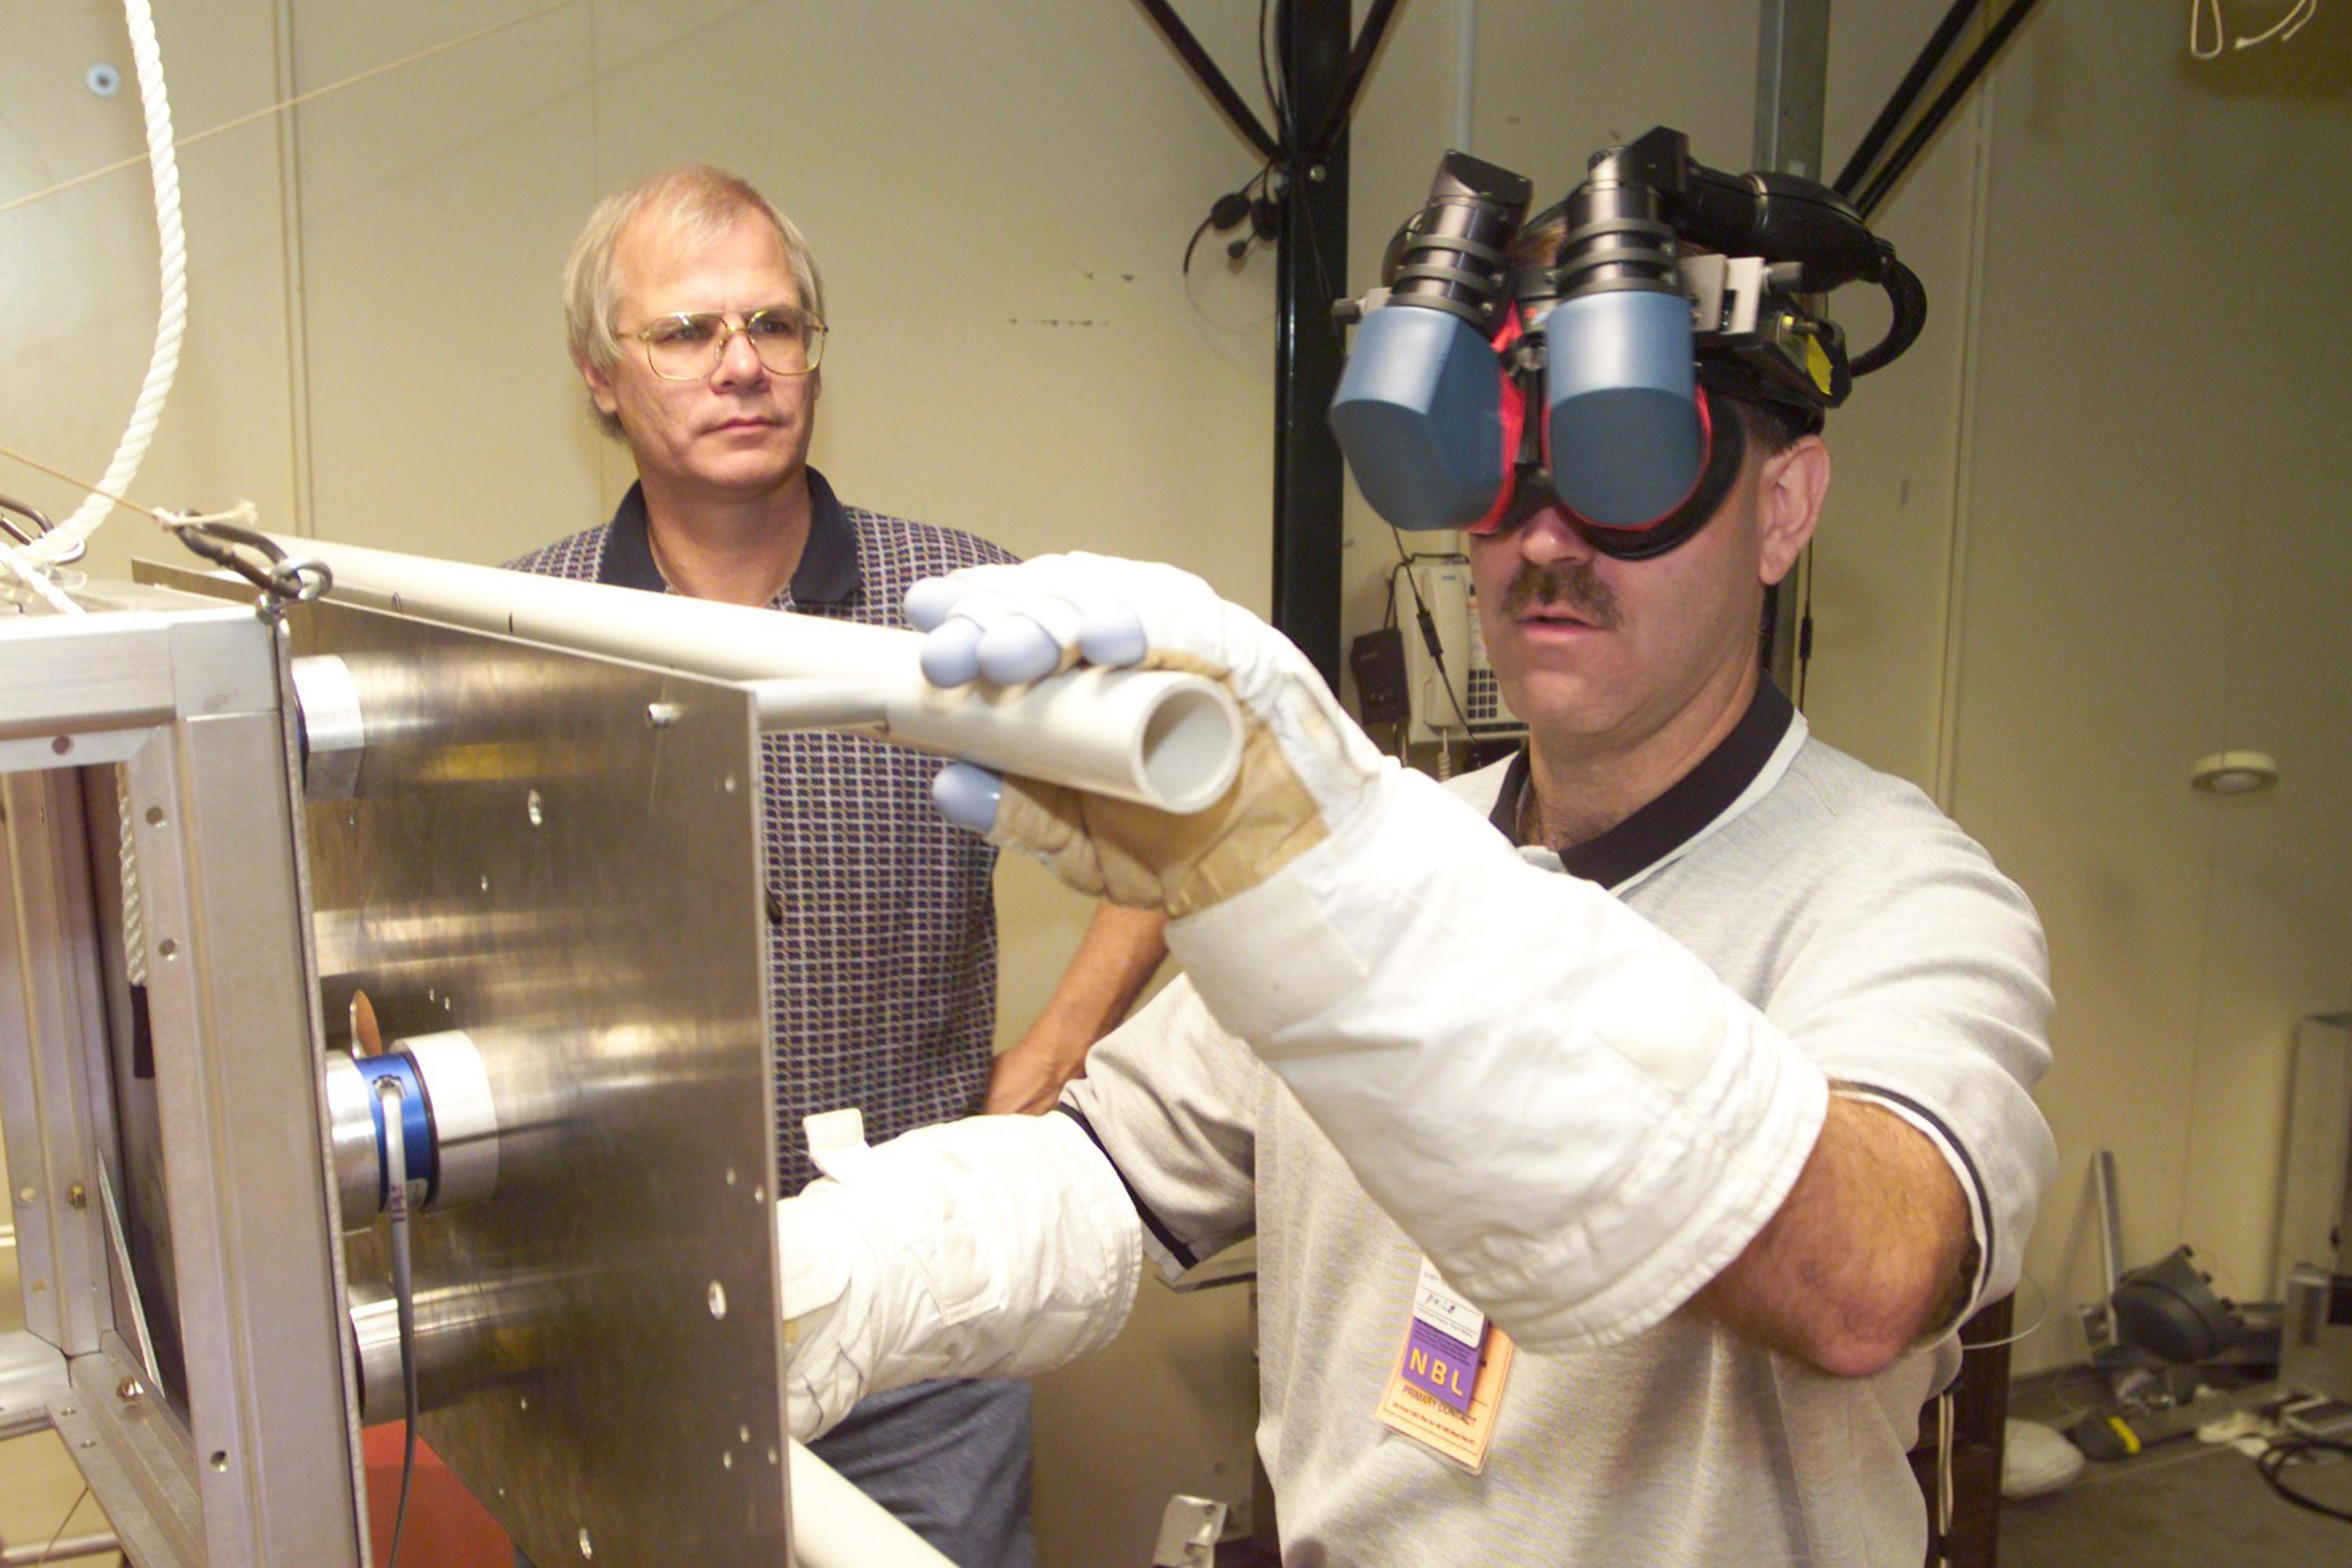
\includegraphics[width=0.45\textwidth]{figures/future-mill.jpg}
  \caption{Grad student tests new virtual reality mill}
  \label{fig:vr-mill}
\end{figure}

\subsection{Subvert Academic Thought}
\todo{Pivot academic thought away from mathematical and computational problems.
Wasted  brainpower when they could be thinking about products and brands.}

\subsection{ACM Seizes Means of Production}
\todo{By putting crushed crystals in CEO's coffee, the ACM will influence CEOs
  to liquidate their companies and give them to the ACM.
  The mills were originally for crushing crystals but after the revolution they
were re purposed to generate electricity
ESPN executives are Mormon though and impervious to crystal healing and coffee. So we had to compromise: the entire National Park System became an ESPN Zone.
}

\subsection{Future Work}
A consequence of the invention of time travel \todo{Cite paper} and the vanity
of engineers (not scientests) \todo{Cite ubiquity article} is that people
keep going further back in time to give themselves credit for the invention of
the time machine.
However, we propose to go back in time for a different reason.
To put a stop to the Open Adcess.
To put a stop to the work dungeons.
And to put a stop to the ACM Revolution, which however noble in it's initial
goals has become  kinda lame.
We will open a mill based on anarchist principles that welcomes all to come and
mill and share healing crystals.
Our report of our screwing missadventuresduring our fieldtrip into the past can
be seen here: \todo{Citation to future article: 1984 esque ACM IS EVERYWHERE,
ACM IS UBIQUITY, WE LOVE ACM}
ubiquity paper}

\todo{Servers powered by manual labor (guy in basement pushing bar around).  If
you want an ad free version you can visit your local ACM work dungeon to
manually turn a generator.)}


\todo{Set system clock to run 10 to the 8 times slower than real time for
reporting performance numbers as recommended by
https://queue.acm.org/detail.cfm?id=3036398}
